\newpage

\section{Odolnost proti násilnému vniknutí}
Základní druhy namáhání, kterým musí trezor odolat, jsou

\begin{itemize}
    \item snaha o~vytržení dveří 
    \item snaha o~odemčení bez znalosti hesla
\end{itemize}

\subsection*{Vytržení dveří}


Jedním ze způsobů~namáhání~mechanizmu~je~vytržení~dveří~z~trezoru.

\paragraph*{Západka}

\begin{figure}[htbp]
    \centering
    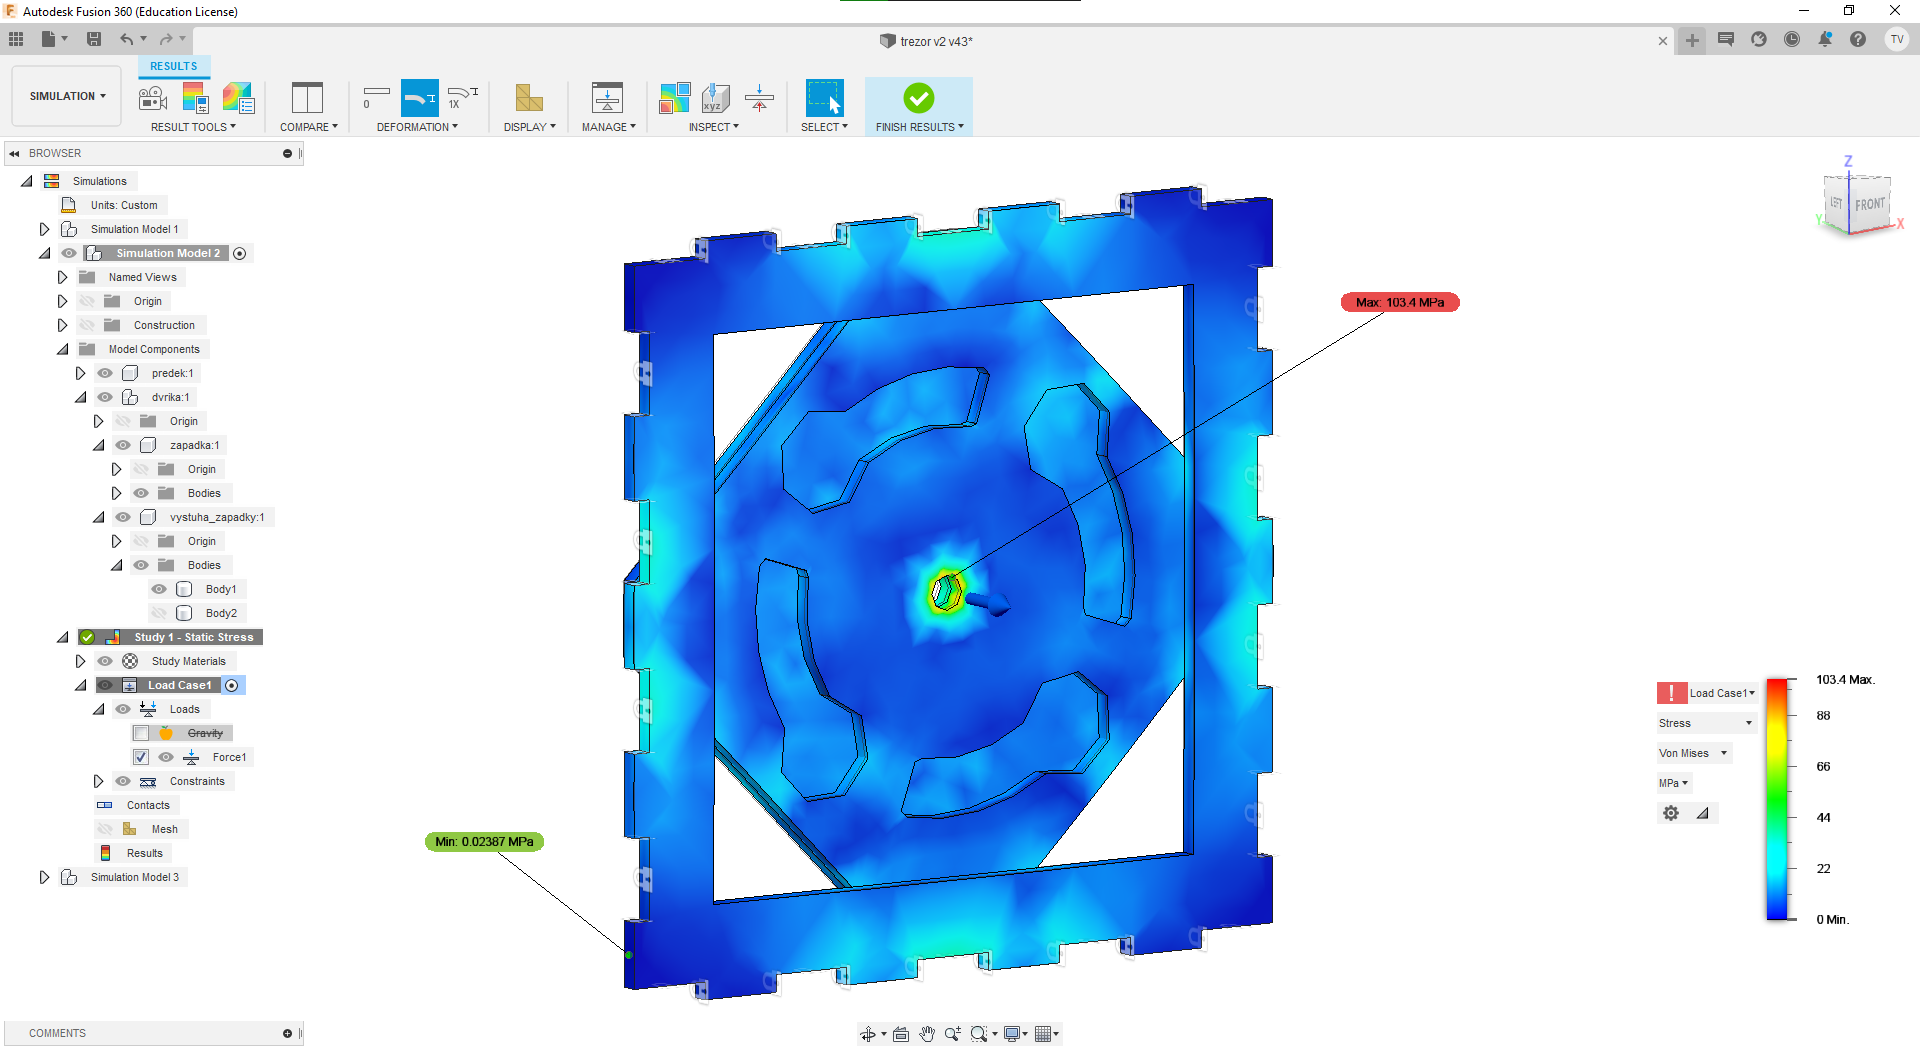
\includegraphics[width=\textwidth]{kapitoly/obrazky/M3/simulace/odolnost_proti_vytrzeni_4kN.png}
    \caption{Simulace pokusu o~vytržení dveří silou 4 000 N}
    \label{fig:M3-simulace-vytrzeni}
\end{figure}
Ze simulace na obrázku \obr{fig:M3-simulace-vytrzeni} vyplývá, že západka odolá pokusu o~vytržení se silou 4~000~N.
%Ke kompletní simulaci se můžete dostat \href{https://myhub.autodesk360.com/ue2d7aa41/g/shares/SH56a43QTfd62c1cd96843f1e03a0eb48053?viewState=NoIgbgDAdAjCA0IDeAdEAXAngBwKZoC40BlASwFsBXAGwEN1SB7AOzXjVoGdPd1C0ARjABsATlEQItALQBjcbmkAWCMIjSBuWgA5lAM22ilAVgAmMAOyy9\%2BBGkYCAVrlnoAkqcIBmAL4gAukA}{zde}
%\parencite{simulase_mechnické} po kliknutí v levém horním rohu na \uv{Simulation} a~\uv{Simulation Model 2}. V~tabulce napravo se pak můžete přepínat mezi barevným zobrazením několika veličin.
%todo opravit odkaz - tohle mi asi nevýjde bohužel ty odkazi nejsou dostupné věčně (jen pár dní) takže to asi Magdě pošlu společně s prací a do SOČky to dávat nemusím vůbec



\begin{table}[h]
    \centering
    \resizebox{0.4\textwidth}{!}{%
    \begin{tabular}{l|l}
    $ \sigma $  & napětí v~materiálu    \\
    $ D $       & průměr kolíku         \\
    $ F $       & působící síla         \\
    $ S $       & plocha průřezu kolíku \\
    \end{tabular}%
    }
    \caption{Tabulka značení veličin pro napětí v~kolíku v~tahu}
    \label{tab:M3_symboly_kolik}
\end{table}

\paragraph*{Kolík}
Při pokusu o~vytržení je celá síla přenášena kolíkem.

\noindent $ \sigma_{max} = 132  $~MPa (\href{https://is.mendelu.cz/eknihovna/opory/zobraz_cast.pl?fit_w=1;cast=9190}{dubové dřevo ve směru vláken při vlhkosti 12 \% }\parencite{pevnost}) % strana 22 tabulka 2 -> https://www.vutbr.cz/www_base/zav_prace_soubor_verejne.php?file_id=66237

\noindent $D = 6$ mm

\noindent \(\sigma_{max} = F/S \Rightarrow F = \sigma_{max} \cdot S~= 132 \cdot (\pi \cdot D^2/4) = 3 732,21 \) N,  z~toho a~ze simulace vyplývá, že kolík je při namáhání nejslabším členem.

\subsection*{Otevření bez odemčení}


Dalším způsobem namáhání může být snaha otočit západkou bez zadání správného hesla.

\paragraph*{Západka}

\begin{figure}[htbp]
    \centering
    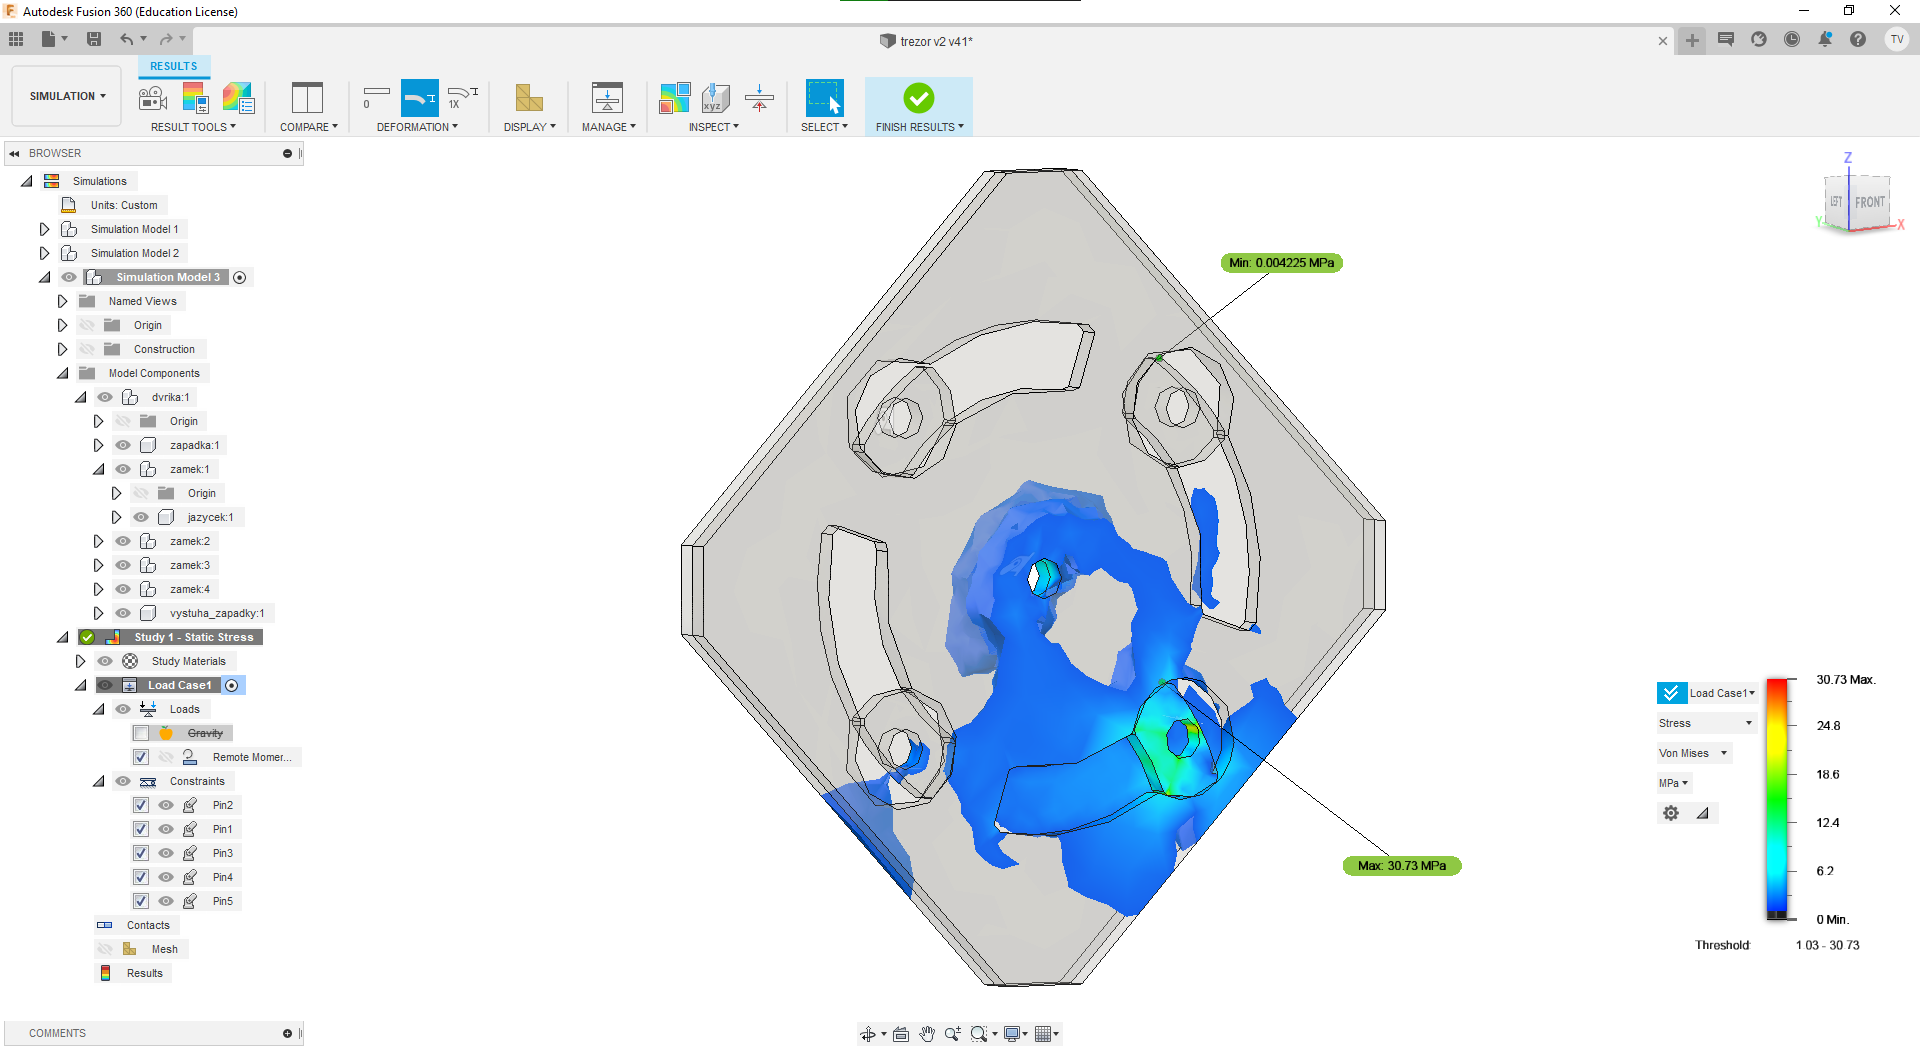
\includegraphics[width=\textwidth]{kapitoly/obrazky/M3/simulace/odolnost_proti_nasilnemu_odemceni_10Nm.png}
    \caption{Simulace pokusu o~otevření bez předchozího odemčení při kroutícím momentu 10 000 N$\cdot$mm, (zobrazeno jen napětí nad 1 MPa) \centering}
    \label{fig:M3-simulace-zapadka}
\end{figure}
Ze simulace na obrázku \obr{fig:M3-simulace-zapadka} vyplývá, že západka odolá pokusu o~otevření bez předchozího odemčení za užití kroutícího momentu o~velikosti 10~000~N$\cdot$mm.
%Ke kompletní simulaci se můžete dostat \href{https://myhub.autodesk360.com/ue2d7aa41/g/shares/SH56a43QTfd62c1cd96843f1e03a0eb48053?viewState=NoIgbgDAdAjCA0IDeAdEAXAngBwKZoC40BlASwFsBXAGwEN1SB7AOzXjVoGdPd1C0ARjABsATlEQItALQBjcbmkAWCMIjSBuWgA5lAM22ilAVgAmMAOyy9\%2BBGkYCAVrlnoAkqcIBmAL4gAukA}{zde}
%po kliknutí v levém horním rohu na \uv{Simulation} a~\uv{Simulation Model 3}. V~tabulce napravo se pak můžete přepínat mezi barevným zobrazení několika veličin.



\begin{table}[h]
    \centering
    \resizebox{0.4\textwidth}{!}{%
    \begin{tabular}{l|l}
    $ \tau $    & napětí v~materiálu při krutu      \\
    $ D    $    & průměr kolíku                     \\
    $ M_k  $    & kroutící moment                   \\
    $ W_k  $    & průřezový modul v~krutu           \\
    \end{tabular}%
    }
    \caption{Tabulka značení veličin pro napětí v~kolíku v~krutu}
    \label{tab:M3_symboly_kolik_otaceni}
\end{table}

\begin{minipage}{\textwidth}
\paragraph*{Kolík}    
Kroutící moment, který je dřevěný kolík o~průměru $D$ = 6~mm schopen přenést. %todo na co tohle navazuje

$ \tau_{max} = 52,3 $ MPa (\href{https://is.mendelu.cz/eknihovna/opory/zobraz_cast.pl?fit_w=1;cast=9190}{dubové dřevo ve směru vláken při vlhkosti 12 \% } \parencite{pevnost})

$ \tau_{max} = \frac{M_k}{W_k} \Rightarrow M_k = \tau_{max} \cdot W_k = \tau _d \cdot \frac{\pi \cdot D^3}{16} $

$ M_k = 52,3 \cdot \frac{\pi \cdot 6^3}{16} = 2 218,16 $ N $\cdot$ mm. Z~výpočtu a~ze simulace plyne, že kolík je při namáhání v~krutu nejslabším místem. Pro zvýšení odolnosti by proto bylo 
potřeba zvětšit kolík nebo změnit materiál.
\end{minipage}